\documentclass[a4paper]{scrartcl}
\usepackage{amsmath}
\usepackage{mathtools}
\usepackage[utf8]{inputenc}
\usepackage[polish]{babel}
\usepackage{textcomp}
\usepackage[T1]{fontenc}
\usepackage{amsthm}
\usepackage{amsfonts}
\newtheorem{definition}{Definicja}
\newtheorem{theorem}{Twierdzenie}
\newtheorem{lemma}{Lemat}
\usepackage{hyperref}
\hypersetup{
    colorlinks,
    citecolor=black,
    filecolor=black,
    linkcolor=black,
    urlcolor=black
}
\usepackage{graphicx}
\title{Sieci komputerowe}
\subtitle{Warsztaty 3}
\author{Dawid Żywczak}
\date{7 kwietnia 2020}

\begin{document}
\maketitle
Ponownie jako dowód rozwiązania zadania, umieszczam zrzuty ekranu historii terminala na poszczególnych maszynach, wyników programów traceroute oraz tablice routingu wyświetlone za pomocą polecenie show ip route. Konwencja przy nadawaniu adresów ip, którą przyjąłem to: 192.168.i.j/24 gdzie i jest numerem sieci local, a j jest numerem maszyny wirtualnej. Dla przykładu dla Virbian1 i interfejsu local0 jest to 192.168.0.1.
Konfigurując protokół RIP (w wersji 2) na maszynach Virbian2, Virbian3, Virbian4, skorzystałem z poniższej serii poleceń (już po uruchomieniu vtysh):\\
1. configure terminal\\
2. router rip\\
3. version 2\\
4. network 192.168.i.0/24 powtórzone dla każdego interfejsu enp-loci\\
\begin{figure}
  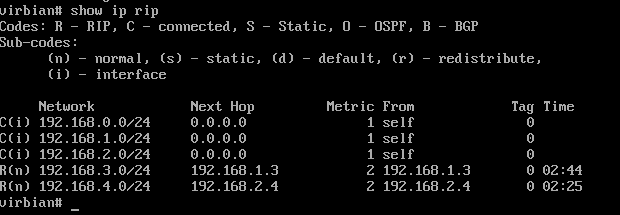
\includegraphics[width=\linewidth]{routingvib2.png}
  \caption{Tablica routingu maszyny Virbian2 po włączeniu protokołu RIP}
\end{figure}
\begin{figure}
  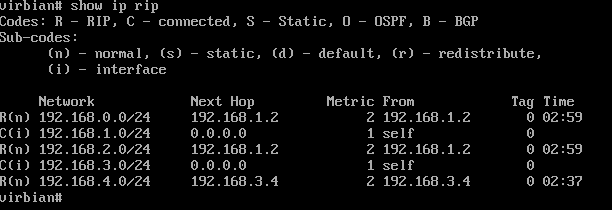
\includegraphics[width=\linewidth]{routingvib3.png}
  \caption{Tablica routingu maszyny Virbian3 po włączeniu protokołu RIP}
\end{figure}
\begin{figure}
  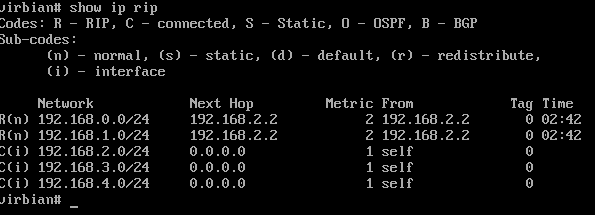
\includegraphics[width=\linewidth]{routingvib4.png}
  \caption{Tablica routingu maszyny Virbian4 po włączeniu protokołu RIP}
\end{figure}
\begin{figure}
  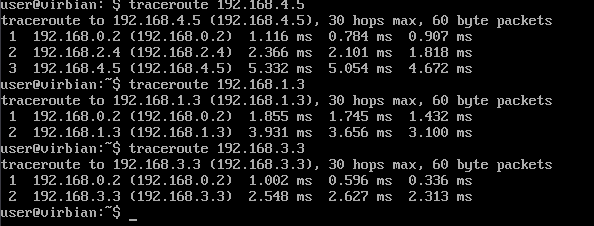
\includegraphics[width=\linewidth]{trvib1.png}
  \caption{Wynik programu traceroute dla maszyny Virbian1 po wykonaniu poleceń}
\end{figure}
\begin{figure}
  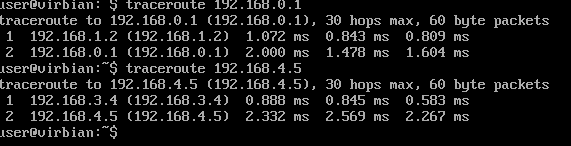
\includegraphics[width=\linewidth]{trvib3.png}
  \caption{Wynik programu traceroute dla maszyny Virbian3 po wykonaniu poleceń}
\end{figure}
\begin{figure}
  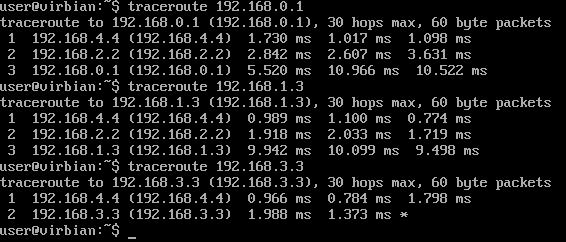
\includegraphics[width=\linewidth]{trvib5.png}
  \caption{Wynik programu traceroute dla maszyny Virbian5 po wykonaniu poleceń}
\end{figure}
\begin{figure}
  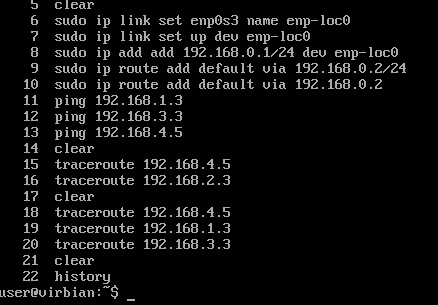
\includegraphics[width=\linewidth]{hvib1.png}
  \caption{Historia terminala dla maszyny Virbian1}
\end{figure}
\begin{figure}
  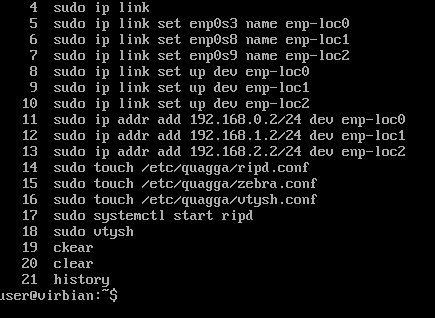
\includegraphics[width=\linewidth]{hvib2.png}
  \caption{Historia terminala dla maszyny Virbian2}
\end{figure}
\begin{figure}
  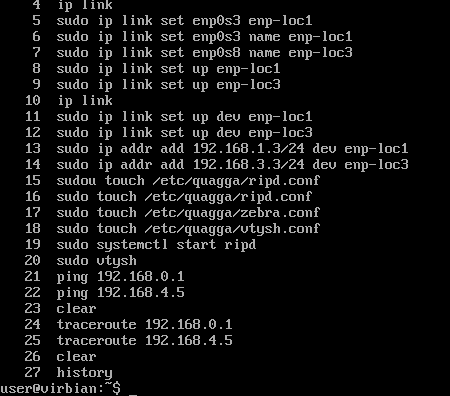
\includegraphics[width=\linewidth]{hvib3.png}
  \caption{Historia terminala dla maszyny Virbian3}
\end{figure}
\begin{figure}
  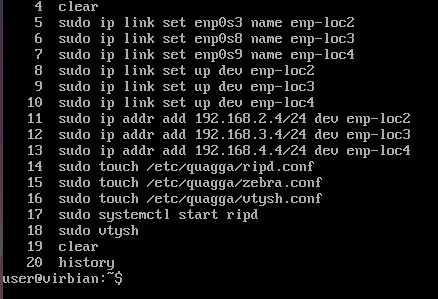
\includegraphics[width=\linewidth]{hvib4.png}
  \caption{Historia terminala dla maszyny Virbian4}
\end{figure}
\begin{figure}
  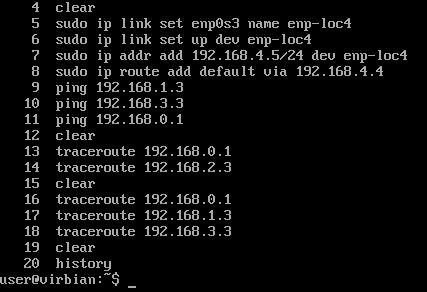
\includegraphics[width=\linewidth]{hvib5.png}
  \caption{Historia terminala dla maszyny Virbian5}
\end{figure}
\end{document}